% Options for packages loaded elsewhere
\PassOptionsToPackage{unicode}{hyperref}
\PassOptionsToPackage{hyphens}{url}
\documentclass[
  12pt,
  a4paperpaper,
]{report}
\usepackage{xcolor}
\usepackage{amsmath,amssymb}
\setcounter{secnumdepth}{5}
\usepackage{iftex}
\ifPDFTeX
  \usepackage[T1]{fontenc}
  \usepackage[utf8]{inputenc}
  \usepackage{textcomp} % provide euro and other symbols
\else % if luatex or xetex
  \usepackage{unicode-math} % this also loads fontspec
  \defaultfontfeatures{Scale=MatchLowercase}
  \defaultfontfeatures[\rmfamily]{Ligatures=TeX,Scale=1}
\fi
\usepackage{lmodern}
\ifPDFTeX\else
  % xetex/luatex font selection
\fi
% Use upquote if available, for straight quotes in verbatim environments
\IfFileExists{upquote.sty}{\usepackage{upquote}}{}
\IfFileExists{microtype.sty}{% use microtype if available
  \usepackage[]{microtype}
  \UseMicrotypeSet[protrusion]{basicmath} % disable protrusion for tt fonts
}{}
\makeatletter
\@ifundefined{KOMAClassName}{% if non-KOMA class
  \IfFileExists{parskip.sty}{%
    \usepackage{parskip}
  }{% else
    \setlength{\parindent}{0pt}
    \setlength{\parskip}{6pt plus 2pt minus 1pt}}
}{% if KOMA class
  \KOMAoptions{parskip=half}}
\makeatother
\usepackage{color}
\usepackage{fancyvrb}
\newcommand{\VerbBar}{|}
\newcommand{\VERB}{\Verb[commandchars=\\\{\}]}
\DefineVerbatimEnvironment{Highlighting}{Verbatim}{commandchars=\\\{\}}
% Add ',fontsize=\small' for more characters per line
\newenvironment{Shaded}{}{}
\newcommand{\AlertTok}[1]{\textcolor[rgb]{1.00,0.00,0.00}{\textbf{#1}}}
\newcommand{\AnnotationTok}[1]{\textcolor[rgb]{0.38,0.63,0.69}{\textbf{\textit{#1}}}}
\newcommand{\AttributeTok}[1]{\textcolor[rgb]{0.49,0.56,0.16}{#1}}
\newcommand{\BaseNTok}[1]{\textcolor[rgb]{0.25,0.63,0.44}{#1}}
\newcommand{\BuiltInTok}[1]{\textcolor[rgb]{0.00,0.50,0.00}{#1}}
\newcommand{\CharTok}[1]{\textcolor[rgb]{0.25,0.44,0.63}{#1}}
\newcommand{\CommentTok}[1]{\textcolor[rgb]{0.38,0.63,0.69}{\textit{#1}}}
\newcommand{\CommentVarTok}[1]{\textcolor[rgb]{0.38,0.63,0.69}{\textbf{\textit{#1}}}}
\newcommand{\ConstantTok}[1]{\textcolor[rgb]{0.53,0.00,0.00}{#1}}
\newcommand{\ControlFlowTok}[1]{\textcolor[rgb]{0.00,0.44,0.13}{\textbf{#1}}}
\newcommand{\DataTypeTok}[1]{\textcolor[rgb]{0.56,0.13,0.00}{#1}}
\newcommand{\DecValTok}[1]{\textcolor[rgb]{0.25,0.63,0.44}{#1}}
\newcommand{\DocumentationTok}[1]{\textcolor[rgb]{0.73,0.13,0.13}{\textit{#1}}}
\newcommand{\ErrorTok}[1]{\textcolor[rgb]{1.00,0.00,0.00}{\textbf{#1}}}
\newcommand{\ExtensionTok}[1]{#1}
\newcommand{\FloatTok}[1]{\textcolor[rgb]{0.25,0.63,0.44}{#1}}
\newcommand{\FunctionTok}[1]{\textcolor[rgb]{0.02,0.16,0.49}{#1}}
\newcommand{\ImportTok}[1]{\textcolor[rgb]{0.00,0.50,0.00}{\textbf{#1}}}
\newcommand{\InformationTok}[1]{\textcolor[rgb]{0.38,0.63,0.69}{\textbf{\textit{#1}}}}
\newcommand{\KeywordTok}[1]{\textcolor[rgb]{0.00,0.44,0.13}{\textbf{#1}}}
\newcommand{\NormalTok}[1]{#1}
\newcommand{\OperatorTok}[1]{\textcolor[rgb]{0.40,0.40,0.40}{#1}}
\newcommand{\OtherTok}[1]{\textcolor[rgb]{0.00,0.44,0.13}{#1}}
\newcommand{\PreprocessorTok}[1]{\textcolor[rgb]{0.74,0.48,0.00}{#1}}
\newcommand{\RegionMarkerTok}[1]{#1}
\newcommand{\SpecialCharTok}[1]{\textcolor[rgb]{0.25,0.44,0.63}{#1}}
\newcommand{\SpecialStringTok}[1]{\textcolor[rgb]{0.73,0.40,0.53}{#1}}
\newcommand{\StringTok}[1]{\textcolor[rgb]{0.25,0.44,0.63}{#1}}
\newcommand{\VariableTok}[1]{\textcolor[rgb]{0.10,0.09,0.49}{#1}}
\newcommand{\VerbatimStringTok}[1]{\textcolor[rgb]{0.25,0.44,0.63}{#1}}
\newcommand{\WarningTok}[1]{\textcolor[rgb]{0.38,0.63,0.69}{\textbf{\textit{#1}}}}
\usepackage{longtable,booktabs,array}
\usepackage{calc} % for calculating minipage widths
% Correct order of tables after \paragraph or \subparagraph
\usepackage{etoolbox}
\makeatletter
\patchcmd\longtable{\par}{\if@noskipsec\mbox{}\fi\par}{}{}
\makeatother
% Allow footnotes in longtable head/foot
\IfFileExists{footnotehyper.sty}{\usepackage{footnotehyper}}{\usepackage{footnote}}
\makesavenoteenv{longtable}
\usepackage{graphicx}
\makeatletter
\newsavebox\pandoc@box
\newcommand*\pandocbounded[1]{% scales image to fit in text height/width
  \sbox\pandoc@box{#1}%
  \Gscale@div\@tempa{\textheight}{\dimexpr\ht\pandoc@box+\dp\pandoc@box\relax}%
  \Gscale@div\@tempb{\linewidth}{\wd\pandoc@box}%
  \ifdim\@tempb\p@<\@tempa\p@\let\@tempa\@tempb\fi% select the smaller of both
  \ifdim\@tempa\p@<\p@\scalebox{\@tempa}{\usebox\pandoc@box}%
  \else\usebox{\pandoc@box}%
  \fi%
}
% Set default figure placement to htbp
\def\fps@figure{htbp}
\makeatother
\ifLuaTeX
\usepackage[bidi=basic]{babel}
\else
\usepackage[bidi=default]{babel}
\fi
\babelprovide[main,import]{ngerman}
% get rid of language-specific shorthands (see #6817):
\let\LanguageShortHands\languageshorthands
\def\languageshorthands#1{}
\ifLuaTeX
  \usepackage[german]{selnolig} % disable illegal ligatures
\fi
\setlength{\emergencystretch}{3em} % prevent overfull lines
\providecommand{\tightlist}{%
  \setlength{\itemsep}{0pt}\setlength{\parskip}{0pt}}
% Table of contents formatting
\renewcommand{\contentsname}{Table of Contents}
\setcounter{tocdepth}{3}

% Number of the last page in the document
\usepackage{lastpage}

% Headers and page numbering
\usepackage{fancyhdr}
\pagestyle{fancy}
\fancyhf{}
\lhead{\rightmark}
\rhead{\thepage\space von \pageref{LastPage}}
\renewcommand{\headrulewidth}{1pt}
\renewcommand{\footrulewidth}{1pt}
\setlength\voffset{0.25in}

% Following package is used to add background image to front page
\usepackage{wallpaper}

% Table package
\usepackage{ctable}% http://ctan.org/pkg/ctable

% Deal with 'LaTeX Error: Too many unprocessed floats.'
\usepackage{morefloats}
% or use \extrafloats{100}
% add some \clearpage

% % Chapter header
\usepackage{titlesec, blindtext, color}
\definecolor{gray75}{gray}{0.75}
\newcommand{\hsp}{\hspace{20pt}}
\titleformat{\chapter}[hang]{\Huge\bfseries}{\thechapter\hsp\textcolor{gray75}{|}\hsp}{0pt}{\Huge\bfseries}

% FONTS
\usepackage{xunicode}
\usepackage{xltxtra}
\defaultfontfeatures{Mapping=tex-text} % converts LaTeX specials (``quotes'' --- dashes etc.) to unicode

%Attempt to set math size
%First size must match the text size in the document or command will not work
%\DeclareMathSizes{display size}{text size}{script size}{scriptscript size}.
\DeclareMathSizes{12}{13}{7}{7}

% Set figure legends and captions to be smaller sized sans serif font
\usepackage[font={footnotesize,sf}]{caption}

\usepackage{siunitx}

% Adjust spacing between lines to 1.5
\usepackage{setspace}
\onehalfspacing
% \doublespacing
\raggedbottom

% Set margins
% \usepackage[top=2cm,bottom=2.5cm,left=3.5cm,right=2.5cm]{geometry}
% \setlength\parindent{0.4in} % indent at start of paragraphs (set to 0.3?)

% Add space between pararaphs
% http://texblog.org/2012/11/07/correctly-typesetting-paragraphs-in-latex/
\setlength{\parskip}{9pt}


% Tables
\usepackage{booktabs}
\usepackage{threeparttable}
\usepackage{array}
\newcolumntype{x}[1]{%
>{\centering\arraybackslash}m{#1}}%

% Allow for long captions and float captions on opposite page of figures
% \usepackage[rightFloats, CaptionBefore]{fltpage}

% Don't let floats cross subsections
% \usepackage[section,subsection]{extraplaceins}
\usepackage{bookmark}
\IfFileExists{xurl.sty}{\usepackage{xurl}}{} % add URL line breaks if available
\urlstyle{same}
\hypersetup{
  pdflang={de-DE},
  hidelinks,
  pdfcreator={LaTeX via pandoc}}

\author{}
\date{}

\begin{document}

\newcommand{\titel}{Entwicklung einer API-basierten Suchfunktion zur Vereinigung mehrerer Datenquellen in der "My BMW" App}
\newcommand{\datum}{xx.xx.xxxx}

\newcommand{\aVorname}{Helena}
\newcommand{\aNachname}{Berndt}
\newcommand{\aGeburtsdatum}{01.03.2002}
\newcommand{\aInstitution}{Hochschule München}
\newcommand{\aStudiengruppe}{IF7}
\newcommand{\aSemester}{WS 2024/2025}

\newcommand{\aName}{\aVorname\space \aNachname}

\newcommand{\pTitle}{Prof. Dr.}
\newcommand{\pVorname}{Lars}
\newcommand{\pNachname}{Wischhof}
\newcommand{\pInstitution}{Hochschule München}

\newcommand{\bTitle}{}
\newcommand{\bVorname}{Daniel}
\newcommand{\bNachname}{Abram}
\newcommand{\bInstitution}{BMW Group}

\title{Entwicklung einer API-basierten Suchfunktion zur Vereinigung mehrerer Datenquellen in der "My BMW" App}
\author{Helena\space Berndt}

\begin{titlepage}
    \begin{center}

        \includegraphics[width=1\textwidth]{style/hm-fk07_logo.jpg}

        \vspace*{1.0cm}

        \LARGE
        Entwicklung einer API-basierten Suchfunktion zur Vereinigung mehrerer Datenquellen in der "My BMW" App

        \vspace{1.5cm}

        \Large
        Helena\space Berndt

        \vspace{0.5cm}

        \normalsize
        Bachelorarbeit Informatik

        \vfill

        \normalsize
        Prüfer:\\
        Prof. Dr.\space Lars\space Wischhof,\space Hochschule München

        \vspace{0.5cm}

        Firmenlogo
        % \includegraphics[width=0.4\textwidth]{style/firmenlogo.png}

        \normalsize
        Betreuer:\\
        \space Daniel\space Abram,\space BMW Group

        % Abgabedatum
        xx.xx.xxxx

    \end{center}
\end{titlepage}

\chapter*{Erklärung}

\begin{center}
  Helena\space Berndt, geb. 01.03.2002\space (IF7,\space WS 2024/2025)
\end{center}

\vspace*{1.0cm}

\noindent Hiermit erkläre ich, dass ich die Bachelorarbeit selbständig
verfasst, noch nicht anderweitig für Prüfungszwecke vorgelegt, keine
anderen als die angegebenen Quellen oder Hilfsmittel benutzt sowie
wörtliche und sinngemäße Zitate als solche gekennzeichnet habe.

\vspace*{1.0cm}

München, xx.xx.xxxx

\vspace*{1.0cm}

\dotfill

Unterschrift \vspace*{\fill} \pagenumbering{gobble}

\chapter*{Zusammenfassung}\label{zusammenfassung}
\addcontentsline{toc}{chapter}{Zusammenfassung}

Lorem ipsum dolor sit amet, consectetur adipiscing elit. Nam et turpis
gravida, lacinia ante sit amet, sollicitudin erat. Aliquam efficitur
vehicula leo sed condimentum. Phasellus lobortis eros vitae rutrum
egestas. Vestibulum ante ipsum primis in faucibus orci luctus et
ultrices posuere cubilia Curae; Donec at urna imperdiet, vulputate orci
eu, sollicitudin leo. Donec nec dui sagittis, malesuada erat eget,
vulputate tellus. Nam ullamcorper efficitur iaculis. Mauris eu vehicula
nibh. In lectus turpis, tempor at felis a, egestas fermentum massa.

\pagenumbering{roman}
\setcounter{page}{1}

\newpage

\chapter*{Danksagungen}\label{danksagungen}
\addcontentsline{toc}{chapter}{Danksagungen}

Interdum et malesuada fames ac ante ipsum primis in faucibus. Aliquam
congue fermentum ante, semper porta nisl consectetur ut. Duis ornare sit
amet dui ac faucibus. Phasellus ullamcorper leo vitae arcu ultricies
cursus. Duis tristique lacus eget metus bibendum, at dapibus ante
malesuada. In dictum nulla nec porta varius. Fusce et elit eget sapien
fringilla maximus in sit amet dui.

Mauris eget blandit nisi, faucibus imperdiet odio. Suspendisse blandit
dolor sed tellus venenatis, venenatis fringilla turpis pretium. Donec
pharetra arcu vitae euismod tincidunt. Morbi ut turpis volutpat,
ultrices felis non, finibus justo. Proin convallis accumsan sem ac
vulputate. Sed rhoncus ipsum eu urna placerat, sed rhoncus erat
facilisis. Praesent vitae vestibulum dui. Proin interdum tellus ac velit
varius, sed finibus turpis placerat.

\pagenumbering{roman}
\setcounter{page}{2}

\newpage

\pagenumbering{gobble}

\rhead{}

\tableofcontents

\newpage

\rhead{\thepage\space von \pageref{LastPage}}

\chapter*{Abbildungsverzeichnis}\label{abbildungsverzeichnis}
\addcontentsline{toc}{chapter}{Abbildungsverzeichnis}

\renewcommand{\listfigurename}{}

\listoffigures

\pagenumbering{roman}
\setcounter{page}{3}

\newpage

\chapter*{Tabellenverzeichnis}\label{tabellenverzeichnis}
\addcontentsline{toc}{chapter}{Tabellenverzeichnis}

\renewcommand{\listtablename}{}

\listoftables

\newpage

\chapter*{Abkürzungsverzeichnis}\label{abkuxfcrzungsverzeichnis}
\addcontentsline{toc}{chapter}{Abkürzungsverzeichnis}

\begin{tabbing}
\textbf{API}~~~~~~~~~~~~ \= \textbf{A}pplication \textbf{P}rogramming \textbf{I}nterface \\  
\textbf{CRUD} \> \textbf{C}reate \textbf{R}ead \textbf{U}pdate \textbf{D}elete \\
\textbf{JSON} \> \textbf{J}ava\textbf{S}cript \textbf{O}bject \textbf{N}otation \\ 
\textbf{REST} \> \textbf{RE}presentational \textbf{S}tate \textbf{T}ransfer \\
\textbf{SDK} \> \textbf{S}oftware \textbf{D}evelopment \textbf{K}it \\
\textbf{URL} \> \textbf{U}niform \textbf{R}esource \textbf{L}ocator \\
\end{tabbing}

\newpage
\setcounter{page}{1}
\renewcommand{\thepage}{\arabic{page}}

\chapter{Einleitung}\label{einleitung}

„\emph{Mit der neuen App-Generation gehen wir einen weiteren Schritt in
der Gestaltung des digitalen Kundenerlebnisses rund um unsere Fahrzeuge
{[}\ldots{]}. Mit der My BMW App {[}\ldots{]} integrieren wir unsere
Fahrzeuge nahtlos in den digitalen Lifestyle unserer Kunden.}`` Mit
diesen Worte des damaligen Senior Vice President der `Connected Company'
der BMW Group, Peter Henrich, wurde die MyBMW App im Jahr 2020 auf den
Markt eingeführt. {[}@koenigYourWorldMy2020{]}

\section{Hintergrund}\label{hintergrund}

Die BMW Group ist ein renommiertes Unternehmen der Automobilindustrie,
das sich auf die Produktion von Fahrzeugen der Premiumklasse fokussiert.
Das Portfolio der BMW Group umfasst die Marken BMW, Mini, Rolls Royce
und BMW Motorrad. {[}@BMWGeschichte{]},
{[}@tholundUmfangreicheUpdatesMy2024{]} Die BMW Group ist u.a. mit einer
Absatzrate von 2,5 Millionen Autos im Jahr 2023 ein signifikanter Faktor
für den Wohlstand Europas {[}@bmwgroupJahresbericht20242024{]}. Der
Automobilsektor trägt mit einem Anteil von 6,1\thinspace\% zur gesamten
Beschäftigung in der EU bei {[}@AutomotiveIndustryEuropean{]} und
generiert etwa 7\thinspace\% des BIP in Europa
{[}@miguelImpactDynamicCapabilities2022{]}.

Der allgemeine Trend der Digitalisierung zeichnet sich auch in der
Automobilindustrie ab. Das digitale Erlebnis eines Produktes ist für
Marken zu einem entscheidenden Unterscheidungsmerkmal geworden
{[}@strategy\&DigitalAutoReport{]}. Es wird prognostiziert, dass
Geschäftsmodelle, wie etwa Konnektivitätsdienste die Einnahmequellen um
etwa 30\thinspace\% steigern könnten
{[}@gaoUmsatzAutoindustrieKann2024{]},
{[}@deryabinaImpactDigitalTransformation2022{]}. Im Bezug auf diese
Entwicklung haben bereits alle Premiumhersteller auf die Entwicklung
reagiert und investieren nun u.a. in die Entwicklung und Bereitstellung
vonApps, die oftmals Remote-Funktionen anbieten und es ermöglichen, auf
das Auto und dessen Daten über ein Handy zuzugreifen
{[}@mollerMobileAppsConnected2019{]}. Daraus resultieren auch
Geschäftsstrategien, die eine detaillierte Analyse der Kundendaten
ermöglichen, um personalisierte Lösungen zu entwickeln
{[}@deryabinaImpactDigitalTransformation2022{]}.

\section{Motivation}\label{motivation}

Die Entwicklung und der Vertrieb von Apps stellen eine Möglichkeit dar,
digitale Innovationen zu fördern, wie es die BMW Group mit der MyBMW App
bereits umgesetzt hat. Diese Applikation bietet den Kunden eine
universelle Schnittstelle zu ihrem Fahrzeug sowie zu einer Vielzahl
weiterer Produkte und Dienstleistungen von BMW
{[}@bmwgroupHighlightsMyBMW{]}.

Die Bereitstellung einer mobilen Anwendung knüpft an eine Entwicklung
an, in der die Bedeutung von Apps kontinuierlich zunimmt. Weltweit
nutzen mehr als drei Viertel der über 10-jährigen Bevölkerung ein
Mobiltelefon, in Europa sind es 93\thinspace\%
{[}@MeasuringDigitalDevelopment{]}. Die Anzahl der jährlichen Downloads
von Apps hat sich zwischen den Jahren 2018 und 2023 mehr als verdoppelt
und steigt weiterhin an {[}@jeanrenaudGlobaleAusgabenFuer2023{]}.

Der Wettbewerb auf dem App-Markt ist sehr intensiv. Einige wenige Apps
dominieren den Großteil des Marktes, was sich daran zeigt, dass Nutzer
bis zu 95\thinspace\% ihrer Zeit mit ihren persönlichen Top-10-Apps
verbringen {[}@martinGlobalMobileReport2017{]}. Insgesamt sind Apps zum
Hauptkonsumenten von internetbasierten Diensten geworden
{[}@maMashDroidApproach2015{]}.

Die zuvor dargestellten Punkte verdeutlichen die Notwendigkeit, dass
insbesondere Unternehmen der Automobilindustrie die Entwicklung von Apps
vorantreiben müssen, um ihre Kunden zu überzeugen. Dabei ist auch die
kontinuierliche Weiterentwicklung der Apps mit der Einführung neuer
Funktionen von entscheidender Bedeutung, um das Kundenerlebnis
langfristig zu optimieren und die Kundenzufriedenheit zu erhöhen. Die
Implementierung einer Suchfunktion ist eine Methode zur Optimierung
einer mobilen Anwendung. Sie ermöglicht es Kunden, Inhalte innerhalb der
App effizienter zu finden, was zu einer Verbesserung des
Nutzungserlebnisses und der Benutzerzufriedenheit führt.

\section{Ziele dieser Bachelorarbeit}\label{ziele-dieser-bachelorarbeit}

\begin{itemize}
\tightlist
\item
  Forschungsfrage ○ Worum geht es in der wissenschaflichten Arbeit? ○
  Was will ich aufzeigen? ○ Warum ist dies wichtig? (Relevanz) ○ Was
  will ich damit erreichen? (Ziel) - Formulierung mit Thema,
  Forschungsfrage, Ziel oder Berechtigung der Forschungsfrage (Ich
  untersuche den Zusammenhang zwischen Studienzufriedenheit und
  Prüfungsleis‐ tungen bei angehenden Absolventen {[}Thema{]}. Damit
  will ich herausfinden, wie sich die Zufriedenheit auf die Leistungen
  von Studierenden in dem letzten Studiensemester bei verschiedenen
  Prüfungsformen auswirkt {[}Forschungsfrage{]}. Daraus sollen konkrete
  Maßnahmen für Studierende und Absolventen abgeleitet werden, um die
  Prüfungsleis‐ tung zu optimieren {[}Ziel oder Berechtigung der
  Forschungsfrage{]}. Leitfragen für Forschungsfragen: für Gestaltung
  -\textgreater{} Welche Massnahmen können ergriffen werden, um ein Ziel
  zu erreichen?
\end{itemize}

Erstellung prototypischer Suchfunktion, die exemplarisch mehrere Quellen
vereint und so durchsuchbar macht. Diese Ansätze bieten eine Grundlage
für eine App-umfassende Suchfunktion.

\section{Abgrenzung}\label{abgrenzung}

Nur 3 Quellen, kein Fokus auf UI

Bei dem Begriff Suchfunktionen wird in dieser Arbeit davon ausgegangen,
dass die Inhalte einer App durchsucht werden. Also beispielsweise die
Texte, die in einer Seite vorkommen. Es soll nicht um die Suche durch
dynamische Inhalte wie zum Beispiel bei YouTube gehen.

\section{Aufbau der Arbeit}\label{aufbau-der-arbeit}

Nach einem einführenden ersten Kapitel \ldots{} Kapitel 2: Grundlagen
des Projektumfeldes Kapitel 3: Vorbereitung und Analyse vergleichbarer
existierender Produkte Kapitel 4: Konzeption der Suchfunktion und API
Kapitel 5: Implementierung der API, Suchfunktion und Benutzeroberfläche
Kapitel 6: Anforderungsabgleich, Bewertung und Evaluierung des Konzeptes
der Suchfunktion Kapitel 7: Zusammenfassung der Arbeit und Ausblick

\chapter{Grundlagen}\label{grundlagen}

\section{Suchfunktionen in mobilen
Anwendungen}\label{suchfunktionen-in-mobilen-anwendungen}

In der heutigen Zeit hat die Relevanz von Suchfunktionen in mobilen
Anwendungen signifikant zugenommen, da eine Vielzahl von Nutzern
regelmäßig mit ihren mobilen Geräten nach Produkten, Dienstleistungen
und Informationen sucht. Aufgrund der umfangreichen Datenmengen, die in
Apps bereitgestellt werden, erweist sich eine effektive Suchfunktion als
unerlässlich, da das eigenständige Durchsuchen dieser Informationen
häufig als zu zeitintensiv und ineffizient wahrgenommen wird.
Unternehmen müssen daher sicherstellen, dass ihre mobilen Anwendungen
ihren Kunden ein gutes Such- und Entdeckungserlebnis bieten, um die
Erwartungen der Zielgruppe zu erfüllen {[}@deeBestPracticesInapp2024{]}.

Die Suche in mobilen Anwendungen unterscheidet sich von den
Suchfunktionen in Desktop-Anwendungen. Im Jahr 2012 wurde festgestellt,
dass Nutzer weniger Suchanfragen pro Sitzung stellen, wenn sie ein
Mobiltelefon verwenden, als wenn sie einen Desktop-PC verwenden
{[}@komakiHowDoesMobile2012{]}. Dies deutet darauf hin, dass Nutzer die
mobile Suche als größere Hürde empfinden. Trotzdem besteht ein starker
Konsens darüber, dass mobile Anwendungen die gleichen
Usability-Anforderungen erfüllen sollten wie Desktop-Anwendungen
{[}@gettoStateMobileUX2020{]}.

Bei der mobilen Suche muss die Balance gefunden werden, dem Nutzer die
relevanten, gesuchten Inhalte zu liefern - ihn aber nicht zu
überfordern, was dazu führen kann, dass die Suche verfeinert und
wiederholt werden muss. Es ist sinnvoll, die Benutzerfreundlichkeit
durch Funktionen wie Filter, Rechtschreibfehlertoleranz, Vorschläge und
frühere Suchanfragen zu verbessern. {[}@deeBestPracticesInapp2024{]}

\section{Flutter}\label{flutter}

Die Entwicklung plattformübergreifender Anwendungen ist für Unternehmen
von entscheidender Bedeutung, um die breite Masse an Kunden zu
erreichen. Dies ist jedoch mit einer gewissen Komplexität verbunden, da
die Plattformen iOS und Android, auf denen die Anwendungen ausgeführt
werden, unterschiedliche Funktionalitäten und Anforderungen aufweisen.
Aktuell werden weltweit etwa 70\thinspace\% der Mobiltelefone mit dem
Betriebssystem Android und 29\thinspace\% mit iOS betrieben
{[}@SmartphoneUsageOperating2024{]}. Entwickler benötigen in der Regel
unterschiedliche Fertigkeiten und müssen Apps aufgrund der
unterschiedlichen Plattformen mehrfach erstellen
{[}@tashildarApplicationDevelopmentUsing2020{]}.

Mit Flutter steht Entwicklern ein plattformübergreifendes
Open-Source-Framework zur Verfügung, das die Erstellung hochperformanter
mobiler Anwendungen aus einer einzigen Codebasis für die beiden
Plattformen iOS und Android ermöglicht {[}@flutterFlutterBuildApps{]}.
Die mobile SDK wurde 2015 durch Google angekündigt
{[}@napoliBeginningFlutterHands2019{]} und der erste Release wurde Ende
2018 publiziert {[}@FlutterSDKArchive{]}.

Flutter-Apps werden in der Programmiersprache \emph{Dart} verfasst, die
ursprünglich die Funktion von JavaScript übernehmen sollte und daher
eine der Programmiersprache Java ähnliche Syntax aufweist. Flutter
erleichtert die Entwicklung durch Funktionen und zeitsparende Tools. So
können Entwickler die `just-in-time' Kompilierung verwenden, bei der der
Computercode während der Programmausführung zur Laufzeit kompiliert
wird. Darüber hinaus ermöglicht die `Hot-Reload' Funktion den
Entwicklern, Benutzeroberflächen zu gestalten oder Features
hinzuzufügen, ohne dass diese Änderungen lange neu geladen werden
müssen. Dabei werden die aktualisierten Quelldaten in die laufende Dart
Virtual Machine eingefügt, die die betroffenen Klassen aktualisiert und
den Widget-Tree automatisch neu baut.
{[}@tashildarApplicationDevelopmentUsing2020{]}

BMW hatte in der nativen Entwicklung früherer Anwendungen
Schwierigkeiten, da die Entwicklungsprozesse als zu aufwendig erachtet
wurden. Daher wurde bei der Konzeption einer neuen Anwendung von Beginn
an die Entscheidung getroffen, Flutter als Entwicklungsframework zu
verwenden. Diese Wahl ermöglicht es, die Vorteile der SDK zu nutzen und
eine plattformübergreifende Entwicklung zu realisieren.
{[}@tasiorDevelopersCars{]}

\section{Die MyBMW-App}\label{die-mybmw-app}

Im Jahr 2020 hat die BMW Group die MyBMW- bzw. Mini-App veröffentlicht,
die den Kunden einen digitalen Zugang zu ihrem Fahrzeug ermöglicht. Die
Entwicklung der App basiert auf dem Feedback und den Erkenntnissen aus
dem Nutzerverhalten der Vorgängergenerationen, der BMW i Remote App und
der BMW Connected App. {[}@koenigYourWorldMy2020{]} Derzeit nutzen mehr
als 13 Millionen Nutzer die App. Sie wird etwa fünf Mal im Jahr durch
Updates aktualisiert {[}@tholundUmfangreicheUpdatesMy2024{]}.

Für die Entwicklung der App wurde Flutter verwendet. Auf dieser
Grundlage ist es möglich, die Applikation sowohl für Android und iOS als
auch für die verschiedenen Skins und Regionen mit der gleichen
Code-Basis zu entwickeln und bauen. Die Skins repräsentieren die Marken
BMW, BMW M, Mini und Toyota. Darüber hinaus existieren spezifische
Versionen für vorgegebene Regionen, wie Nordamerika oder Südkorea.
Daraus resultieren ca. 30 Apps, die den Kunden in den Apps Stores
angeboten werden. Das Team von ca. 250 Entwicklern ist eines der größten
Flutter-Entwicklungsteams überhaupt. {[}@tasiorDevelopersCars{]}

Die Applikation stellt dem Kunden eine universelle Schnittstelle zum
Fahrzeug bereit. Mittels dieser Schnittstelle können Remote-Funktionen
ausgeführt werden, womit der Fahrzeug- oder Ladestatus, die Reichweite
sowie die Türen und Fenster des Autos aus der Ferne über das
Mobiltelefon überprüft werden können. Die Funktionsweise ist auf
Fahrzeuge ab dem Baujahr 2014 optimiert und kann sich abhängig von der
Fahrzeugausstattung sowie länderspezifischen Vorgaben unterscheiden.
{[}@bmwgroupHighlightsMyBMW{]}

Nach erfolgter Anmeldung mit der BMW-ID ermöglicht die App den Zugriff
auf das Fahrzeug, BMW-Services und -Store. Die App ist in mehrere
Unterseiten, so genannte Tabs, unterteilt. Im Fahrzeug-Tab erhält der
Kunde einen Überblick über den aktuellen Zustand seines Autos, also
Fahrzeugstatus und Remote-Funktionen. Im Karten-Tab können Ziele zur
Navigation gesucht und ausgewählt werden. Der BMW-Services- und
Store-Tab bietet den Kunden direkten Zugriff auf Updates und
Finanzdienstleistungen und ermöglicht den Kontakt zu Service Partnern.
Im Profil-Tab können persönliche Einstellungen vorgenommen werden.
{[}@bmwHowErsteSchritteMit2024{]}

Ein besonderes Feature ist das Remote Software Upgrade (RSU), mit dem
Updates für die Fahrzeugsoftware direkt `over-the-air' ins Fahrzeug oder
zunächst in die MyBMW-App und dann auf das Auto geladen werden.
{[}@julichUpdateFuerFreude2021{]}

\emph{todo: hier Bilder?}

\section{API-Entwicklung}\label{api-entwicklung}

APIs sind entscheidend für die nahtlose Kommunikation zwischen
Softwarekomponenten und -diensten. Sie sind essenziell für die
Verbindung verschiedener Systeme und ermöglichen die Nutzung von
Diensten, Daten und Funktionalitäten Dritter.
{[}@selvarajMasteringRESTAPIs2024{]}

Mit APIs kann auf unterschiedliche Komponenten zugegriffen werden,
darunter Hardwarekomponenten, Datenbanken, einzelne Programmfunktionen
oder auch Oberflächen.
{[}@luberAPIEntwicklungGrundlagenEigenschaften2024{]}

Der Begriff API ist vielseitig interpretierbar und kann sich auf eine
rein technische Schnittstellenbeschreibung, ein Kommunikationsmittel für
Software oder auch um ein digitales Produkt beziehen. In allen Fällen
sind APIs kein separates Softwaresystem, sondern lediglich eine
Kommunikationsschnittstelle, die der Interaktion mit der Software dient.
{[}@frankBausteineDigitalenTransformation2021{]}

Darüber hinaus wird zwischen funktions-, datei-, objekt- und
protokollorientierten APIs differenziert.
{[}@luberAPIEntwicklungGrundlagenEigenschaften2024{]}

Die Eigenschaften von APIs lassen sich wie folgt zusammenfassen:
Modularität, das heißt die Zusammensetzung eines Services aus mehreren
separaten Services, Interoperabilität, also die Existenz von Standards
in der Kommunikation zwischen Diensten, und die Kapselung, bei der die
Programmlogik und die Datenbasis des Services verborgen bleiben.
{[}@frankBausteineDigitalenTransformation2021{]}

Die Modularisierung von Software führt zur Trennung einzelner
Programmteile, die spezifische Funktionen erfüllen, und zur Trennung vom
Rest der Applikation. Die Kommunikation erfolgt über eine genau
definierte Schnittstelle, was zu einer sauberen Gesamtstruktur innerhalb
des Projektes führt. Dies kann besonders komplexe Programme
vereinfachen. Die einzelnen Programmteile sind leichter wartbar und
damit weniger fehleranfällig.
{[}@luberAPIEntwicklungGrundlagenEigenschaften2024{]}

Die Verwendung von APIs hat sich als signifikant effizienter und
beschleunigender Faktor in der Entwicklung von Anwendungen und Software
erwiesen. Die gemeinsame Nutzung von Daten ermöglicht die Freigabe
spezifischer Informationen, während systeminterne Details verborgen
bleiben, was zu einer Optimierung der Sicherheit und Vertraulichkeit
beiträgt. {[}@ibmWhatAPIApplication2024{]}

Die Implementierung einer API ist ein wesentlicher Faktor für den Erfolg
mobiler Applikationen. Instabilität und Fehleranfälligkeit der API
können den Erfolg der Software erheblich beeinträchtigen. Eine gute API
ist ein wesentlicher Faktor für den Erfolg einer App. Eine Auswertung
von Google Play-Bewertungen hat ergeben, dass erfolgreiche Apps weniger
fehleranfällige APIs verwenden {[}@linares-vasquezAPIChangeFault2013{]}.

\chapter{Vorbereitung und Analyse der
Ausgangssituation}\label{vorbereitung-und-analyse-der-ausgangssituation}

Im Vorfeld der eigentlichen Konzeption der Suchfunktion erfolgt zunächst
eine umfassende Analyse der Ausgangssituation. Zunächst werden
allgemeine Funktionen und Anforderungen zusammengefasst, die
üblicherweise an eine moderne Suchfunktion gestellt werden. Im Anschluss
daran werden vergleichbare Suchfunktionen in Automotive-Apps sowie in
anderen Anwendungsbereichen analysiert und mit den Anforderungen
abgeglichen. Abschließend wird der Ist-Zustand der vorhandenen Daten und
Datenquellen betrachtet.

\section{Allgemeine Funktionen und Anforderungen an eine
Suchfunktion}\label{allgemeine-funktionen-und-anforderungen-an-eine-suchfunktion}

Bei der Entwicklung von Suchfunktionen in mobilen Anwendungen sollten
bewährte Verfahren, auch bekannt als `Best Practices', in die Konzeption
einfließen. Oftmals verfügen Suchfunktionen über einen
Übergangsbildschirm, der vergangene Suchanfragen, trendige Suchbegriffe
oder vordefinierte Kategorien anbietet. Eine Filtermöglichkeit ist
besonders sinnvoll, wenn relevante Daten vorhanden sind. Bei der Eingabe
von Suchbegriffen wird häufig eine Autovervollständigung angeboten, die
Vorschläge für mögliche Suchanfragen liefert. Dabei werden häufig auch
Schreibfehler toleriert, um die Benutzerfreundlichkeit zu erhöhen. In
den Suchergebnissen können die eingegebenen Suchwörter durch eine
Markierung hervorgehoben werden, was die Übersichtlichkeit verbessert.
Die Integration von Künstlicher Intelligenz kann in bestimmten
Anwendungsfällen von Suchfunktionen von Vorteil sein, beispielsweise zur
Schaffung eines personalisierten Einkaufserlebnisses. Letztlich ist es
entscheidend, dass die Erwartungen der Nutzer an die Geschwindigkeit der
Suchfunktion erfüllt werden, um eine positive Benutzererfahrung zu
gewährleisten.{[}@deeBestPracticesInapp2024{]}

Um die Suchfunktion zu starten, kann die Suchleiste entweder durch das
Anklicken eines Suchsymbols aufgerufen oder direkt angezeigt werden.
Wenn die Suche in einer Anwendung im Vordergrund steht, ist es
empfehlenswert, die Suchleiste sofort anzuzeigen. Ist die Suche hingegen
optional, kann ein kontextbezogenes Suchsymbol verwendet werden.
{[}@holstECommerceSearchField2014{]}

Ein weiterer Trend, der sich bei den Suchfunktionen abzeichnet, sind
Sprachfunktionen. So wurden 2016 20\thinspace\% der Google-Suchanfragen
über die Sprachfunktion getätigt {[}@GoogleAppVoice2016{]}. Laut einer
Studie im Jahr 2018 tätigen die Handynutzer mit 27\thinspace\% die
meisten Suchanfragen mit Sprachfunktion bzw. Sprachbefehlen, gefolgt von
Tablet- und PC-Nutzern. Es wurde festgestellt, dass jüngere Nutzer öfter
Sprachsuche oder Sprachbefehl-Tools verwendet haben.
{[}@VoiceSearch2018{]}

\section{Recherche und Analyse vergleichbarer
Suchfunktionen}\label{recherche-und-analyse-vergleichbarer-suchfunktionen}

Im Folgenden werden zunächst Apps von Automobilherstellern, die als
direkte Wettbewerber der MyBMW-App angesehen werden können, näher
betrachtet. Dabei wird ein besonderer Fokus auf eventuell vorhandene
Suchfunktionen gelegt. Anschließend erfolgt eine allgemeine Analyse von
Suchfunktionen in Apps, die einen Überblick über typische Konzepte und
Funktionen liefert.

\subsection{Suchfunktionen in Automotive
Apps}\label{suchfunktionen-in-automotive-apps}

Eine Analyse der von den Automarken Mercedes, Audi, Tesla, Volkswagen
und Volvo angebotenen Apps zeigt, dass sie mit der MyBMW App
vergleichbar sind. Die Untersuchung der Funktionalitäten der
Wettbewerber-Apps ergibt, dass die Grundfunktionen ähnlich sind. Dazu
gehören Remote-Funktionen, mit denen z.B. das aktuelle Klima eingesehen
und gesteuert werden kann, sowie die Möglichkeit, Fahrzeuge über das
Handy zu entriegeln und den Fahrzeugstatus abzurufen. Zusätzlich haben
Kunden die Möglichkeit, den aktuellen Standort des Autos zu überprüfen
und Routen zu planen. Die Analyse der im App Store sichtbaren Funktionen
ergab jedoch, dass keine der untersuchten Apps über eine Suchfunktion
verfügt, die eine Suche nach Stichwörtern ermöglicht.
{[}@AppStoreMercedesBenz2024{]},{[}@AppStoreMyAudi2024{]},{[}@AppStoreTesla2024{]},{[}@AppStoreVolkswagen2024{]},{[}@AppStoreVolvo2024{]}

\emph{todo: diese quellen sind eigene quellen -\textgreater{} in den
anhang?}

\subsection{Suchfunktionen in Apps anderer
Bereiche}\label{suchfunktionen-in-apps-anderer-bereiche}

\emph{ToDo: hier klären, wie diese ``eigenen'' Aufnahmen zitiert werden}
\emph{Todo: hier Bilder einfügen!}

Um einen Überblick über typische Suchfunktionen in mobilen Anwendungen
zu erlangen, werden im Folgenden die Suchfunktionen von Apps aus
verschiedenen Anwendungsbereichen analysiert. Ziel dieser Analyse ist
die Entwicklung eines Verständnis für die Konzepte und Funktionen von
In-App-Suchfunktionen.

Die Suchfunktion der `Einstellungen'-App von Apple für iOS ermöglicht
die Suche nach spezifischen Begriffen, die in das am Seitenanfang
befindliche Suchfeld eingegeben werden. Hierbei durchsucht die App
sämtliche Inhalte der Einstellungen. In der Version der Softwarestufe
iOS 17 werden während der Eingabe Suchergebnisse angezeigt, ohne dass
eine explizite Bestätigung der Eingabe durch den Nutzer erforderlich
ist. Die Suche generiert eine Liste mit treffenden Ergebnissen, wobei
der Titel des zugehörigen Feldes innerhalb der App, ein zugehöriges
Symbol und teilweise der Pfad angegeben werden. Durch Anklicken eines
Ergebnisses wird die entsprechende Seite geöffnet bzw. der gesamte Pfad,
wobei das zugehörige Feld kurzzeitig grau hervorgehoben wird. Navigiert
man zurück, gelangt man, wenn im Pfad vorhanden, auf eine Oberseite,
bevor man wieder auf das Suchfenster zurückkommt.
{[}@EinstellungenAppIPhone2024{]}

Ab iOS 18 werden vor der Eingabe in das Suchfeld Such-Vorschläge durch
große Symbole und Text angezeigt und darunter der Verlauf der
aufgerufenen Suchergebnisse. {[}@EinstellungenAppIPhone2025{]}

Die `Einstellungen'-App von Android kann ebenfalls nach Begriffen
durchsucht werden. Nach Anklicken des Such-Icons wird die Suchseite
geöffnet, in der vergangene Suchen und allgemeine Suchvorschläge
aufgelistet sind. Den Vorschlägen geht ein Rauten-Symbol vor, wodurch
nach Themen und nicht nach konkreten Begriffen gesucht werden kann, wie
etwa ``beliebt''. Während der Eingabe in das Suchfeld werden dann
anstelle dessen die Suchergebnisse für die aktuelle Eingabe angezeigt.
Diese sind in beliebte und restliche Ergebnisse aufgeteilt, die jeweils
in ihre zugehörigen Kategorien gruppiert sind. Durch Anklicken eines
Ergebnisses wird die entsprechende Seite innerhalb der
`Einstellungen'-App geöffnet. Durch Betätigen der `Zurück'-Taste des
Handys, gelangt man in die Suchfunktion. Durch Betätigung des
`Zurück'-Button in der Leiste oben, geht man dem der Seite zugehörigen
Pfad entlang zurück. {[}@EinstellungenAppAndroid{]}

Als weiteres Beispiel bietet die App `Instagram' für ihren
Einstellungen-Bereich eine Suchfunktion an, mit der die Inhalte dieses
Bereiches durchsucht werden können. Bei der Eingabe von Suchbegriffen
werden die Suchergebnisse in verschiedenen Gruppen untereinander bereits
während des Tippens, ohne explizite Bestätigung, angezeigt. Diese
Gruppierung entspricht der Kategorisierung, die in den Einstellungen
verwendet wird. Beim Anklicken eines Ergebnisses wir direkt die
entsprechende Unterseite geöffnet. Es sei jedoch angemerkt, dass nicht
alle in den Einstellungen dargestellten Inhalte durch die Suche
auffindbar sind. {[}@InstagramEinstellungen2025{]}

Die untersuchten Apps setzen viele der zuvor erhobenen Anforderungen um.
Häufig gibt es einen Übergangsbildschirm, der Vorschläge und vergangene
Suchanfragen anzeigt. Während des Tippens werden jedoch oft nur die
Ergebnisse für den aktuellen Stand des Suchbegriffs angezeigt, ohne dass
Vorschläge für eine automatische Vervollständigung angeboten werden.
Zudem wurden die Suchergebnisse auf den Seiten nur teilweise explizit
hervorgehoben. Es besteht auch keine Konsistenz darin, ob die
Suchfunktion über eine Suchleiste oder ein Suchsymbol aufgerufen wird.
Insgesamt zeigen sich sowohl Übereinstimmungen als auch Unterschiede in
den Implementierungen der Suchfunktionen.

\section{Ist-Analyse der vorhandenen Daten und
Datenquellen}\label{ist-analyse-der-vorhandenen-daten-und-datenquellen}

Um eine umfassende Suche durch verschiedene Bereiche der MyBMW-App zu
ermöglichen, werden die Daten aus verschiedenen Quellen angebunden.

Die Texte, die in der MyBMW-App verwendet werden, beispielsweise in
Buttons, Menüpunkten oder anderen Anzeigekomponenten, sind in
sogenannten `String Files' gespeichert. Diese Dateien ermöglichen es,
die Anwendung in verschiedenen Sprachen darzustellen, indem die Texte in
der jeweiligen Sprache aus der entsprechenden Datei geladen werden.
Jeder Text ist mit einer eindeutigen ID versehen, die es ermöglicht, die
Texte den verschiedenen Features innerhalb der App zuzuordnen. Jedes
Feature hat dabei einen zugehörigen Pfad, der dann auf die entsprechende
Seite des Features führt. Im Rahmen der Implementierung der Suchfunktion
sollen exemplarisch zwei Dienste der MyBMW-App an die Suchfunktion
angebunden werden. Diese Daten werden im Weiteren als
\emph{`String-File'-Daten} bezeichnet.

Zusätzlich wird eine dynamische Quelle integriert, die über die App
bereitgestellt und über den `Context' geladen werden kann. Diese Quelle
umfasst die Artikel, die auf der Explore-Seite der MyBMW-App dargestellt
werden, und bietet somit aktuelle Inhalte für die Suche. Diese Daten
werden als \emph{Kontext-Daten} bezeichnet.

Darüber hinaus werden lokale Daten in Form einer JSON-Datei in die Suche
integriert. In dieser prototypischen Umsetzung enthält die JSON-Datei
Datensätze zu `My Highlights', die besondere Änderungen bei RSU für die
Kunden hervorheben. Diese Daten werden als \emph{Lokale-Daten}
referenziert.

\chapter{Konzeption}\label{konzeption}

\emph{todo: Forschungsfrage konkretisieren hier}

\section{Anforderungsanalyse der
Suchfunktion}\label{anforderungsanalyse-der-suchfunktion}

\emph{todo: sollen hier auch nicht-umgesetzte sachen stehen? wenn ja
hier nochmal mehr stukturieren und priorisieren - in must-haves und
nice-to-haves?}

Im `Requirements Engineering', also der Anforderungsanalyse, werden die
Bedürfnisse der Benutzer, Auftraggeber und anderen Interessensgruppen
analysiert, um eine geeignete Lösung für ein Produkt zu entwickeln.
Dabei wird eine Übereinkunft über die Funktionen des Systems, die
Systemgrenzen und die Benutzerschnittstellen getroffen. Diese
Informationen helfen auch den Entwickler, die Anforderungen besser zu
verstehen. Dabei wird zwischen funktionalen und nicht-funktionalen
Anforderungen unterschieden. Die funktionalen Anforderungen beziehen
sich auf Aspekte, die die Funktionalität des Produkts erklären.
Nicht-funktionale Anforderungen beziehen sich auf die erforderlichen
Qualitätsaspekte und Rahmenbedingungen, d.h. Elemente, die für das
Nutzererlebnis eine wichtige Rolle spielen. In der Regel werden die
Inhalte u.a. durch Interviews mit Stakeholdern oder Nutzerbefragungen
ermittelt. {[}@richterUsabilityUndUX2016{]}

Da es sich bei der Entwicklung der Suchfunktion um eine prototypische
Umsetzung handelt, wurde hierfür keine Nutzerbefragung zur Ermittlung
der Anforderungen durchgeführt. Vermutliche Nutzerbedürfnisse wurden
viel mehr antizipiert. Nicht alle an die Suchfunktion gestellten
Anforderungen werden aufgrund des begrenzten Zeitrahmens der
Durchführung der Bachelorarbeit umgesetzt.

\subsection{Systematische Erfassung der
Anforderungen}\label{systematische-erfassung-der-anforderungen}

Die funktionalen Anforderungen sind an die zu entwickelnde Suchfunktion
sind wie folgt definiert:

\begin{itemize}
\tightlist
\item
  Die Suchfunktion soll der bestehenden `Explore'-Seite hinzugefügt
  werden
\item
  Nach dem Anklicken eines Suchsymbols soll der Benutzer einen einzelnen
  Suchbegriff in ein vorgegebenes Suchfeld eingeben können
\item
  Vor der Eingabe einer Suchanfrage in die Suchleiste sollen dem Nutzer
  allgemeine Vorschläge und frühere Suchanfragen angezeigt werden
\item
  Während des Tippens in die Suchleiste sollen Suchvorschläge gegeben
  werden, die das aktuelle Suchwort ergänzen - diese Anforderung wurde
  im Rahmen der Bachelorarbeit nicht umgesetzt
\item
  Bei der Bestätigung eines Begriffs werden die zur Suche verfügbaren
  Quellen über die Schnittstelle durchsucht und anschließend jene
  Ergebnisse angezeigt, die den Suchbegriff beinhalten
\item
  Mithilfe eines Filters können die zu durchsuchenden Quellen bestimmt
  werden - diese Anforderung wurde im Rahmen der Bachelorarbeit nicht
  umgesetzt
\item
  Kleine Rechtschreibfehler oder nicht exakte Übereinstimmungen zwischen
  Suchbegriff und durchsuchten Daten sollen toleriert werden
\item
  Die Resultate der Suche werden in reduzierter Form untereinander
  angezeigt
\item
  Zu jedem Ergebnis werden ein Titel und Ausschnitte eines längeren
  Textes dargestellt. Durch Anklicken wird die dazugehörige Seite
  geöffnet, während beim Verlassen der Seite wieder die Ergebnisse der
  Suchfunktion angezeigt werden
\end{itemize}

Die nicht-funktionalen Anforderungen umfassen:

\begin{itemize}
\tightlist
\item
  Die Suchfunktion soll eine gute Performance aufweisen, d.h. die
  Suchergebnisse sollen schnell angezeigt werden
\item
  Die Suchfunktion soll benutzerfreundlich sein. Bei der prototypischen
  Umsetzung der Suchfunktion im Rahmen dieser Bachelorarbeit steht das
  UX-Design jedoch nicht im Vordergrund
\end{itemize}

Neben der Analyse der Anforderungen an die Suchfunktion, werden auch die
technischen Rahmenbedingungen analysiert. So sollen die technischen
Möglichkeiten und Grenzen untersucht, geeignete Frameworks gefunden und
Schnittstellen geprüft werden. Die Suchfunktion soll in die bestehende
App-Umgebung der MyBMW-App integriert werden. Da die MyBMW-App mit
Flutter entwickelt wurde, basiert die grundlegende technische
Infrastruktur der Suchfunktion auf der Programmiersprache Dart.

Flutter stellt u.a. die Klasse `\emph{SearchDelegate}' zur Verfügung,
die eine Suchseite erzeugt, die u.a. Vorschläge und Ergebnisse anzeigt
und im Code Zugriff auf das aktuelle Suchwort, also `\emph{query}'
ermöglicht {[}@SearchDelegateClassMaterial{]}. Diese Klasse vereint die
genannten Anforderungen. Die Klasse `\emph{SearchBar}' stellt zum
Vergleich nur das Eingabefeld für die Suchbegriffe zur Verfügung
{[}@flutterSearchBarClassMaterial{]}.

Die Datenquellen für die Suchfunktion sind die bereits erwähnten
\emph{`String Files'-}, \emph{Kontext-} und \emph{Lokale-Daten}.

Um letztere Daten aus der lokalen Datei, also der JSON-Datei, lesen zu
können, müssen diese zunächst in ein für Dart lesbares Format gebracht
werden. Dies kann mit dem Dart-Package `\emph{json\_serializable}'
realisiert werden. Damit können Daten zwischen dem JSON-Format und der
gewünschten und durch den Code definierten Struktur konvertiert werden.
{[}@Json\_serializableDartPackage{]}

In allen Quellen werden für die Suchfunktion unterschiedliche Strings
nach Übereinstimmungen durchsucht. Um kleine Abweichungen zwischen Such-
und Vergleichswort zu tolerieren, kann das Dart Package `\emph{Fuzzy}'
verwendet werden. Mit diesem wird ein für einen String-Vergleich ein
sogenannter Fuzzy-Score erzeugt, der angibt, wie groß die
Übereinstimmung ist. {[}@FuzzyDartPackage{]}

\subsection{Konzeptentwurf}\label{konzeptentwurf}

Auf Basis der systematischen Erfassung der Anforderungen an die
Suchfunktion wird nun das Konzept für die Suchfunktion konkretisiert.
Die Konzeption und der Aufbau der API, an die die Suchanfragen gestellt
wird und die die verschiedenen Quellen zusammenführt, werden in Kapitel
\ref{konzeption-der-api} behandelt. Daher wird an dieser Stelle nicht
näher darauf eingegangen. Grob betrachtet schickt die Suchfunktion ein
Suchbegriff an die API und bekommt von dieser dann die Ergebnisse für
die Anfrage zurück. (Siehe Abbildung \ref{fig:suchfunktion_api})

\begin{figure}
\centering
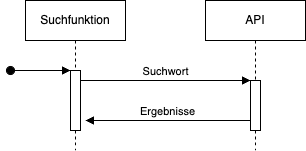
\includegraphics[width=0.5\linewidth,height=\textheight,keepaspectratio]{source/figures/Suchfunktion_API.drawio.png}
\caption{Quelle: eigenes Diagramm, 2025}\label{fig:suchfunktion_api}
\end{figure}

Der Ablauf der Suchfunktion aus Benutzersicht soll wie folgt ablaufen:
Durch Anklicken des Lupensymbols auf der `Explore'-Seite, öffnet sich
die Seite der Suchfunktion. Über die Leiste am oberen Rand dieser Seite
können folgende Funktionen ausgeführt werden: Es besteht die Möglichkeit
zurück zur vorherigen Seite zu navigieren, einen Suchbegriff einzugeben
oder den bisher eingegebenen zu löschen. Unterhalb der Leiste befinden
sich Suchvorschläge, die von der Funktionsseite gegeben werden und die
zuletzt durchgeführten Suchanfragen. Dabei muss entschieden werden, ob
diese Funktionen durch Symbole dargestellt oder mit Text angeschrieben
werden. Auch muss entschieden werden, ob die Suchvorschläge dynamisch
oder statisch sind.

Eine Suchanfrage wird durchgeführt, indem ein Suchbegriff in das
Suchfeld eingegeben und dann mit der Eingabetaste bestätigt wird.
Während des Tippens wird die Seite mit Suchverlauf und den Vorschlägen
weiter angezeigt. Der Suchbegriff wird an die API geschickt, die diese
Anfrage bearbeitet. Anschließend werden die durch die API gefundenen
Ergebnisse nach Relevanz sortiert aufgelistet. Diese können je nach
Quelle und damit Inhalt unterschiedlich aufgebaut sein.

Bei den Ergebnissen aus den `\emph{String-Files}' müssen einige Punkte
bedacht werden. So muss geklärt werden, ob nur die Datei für die
aktuelle Sprache, in der die App gerade ist, oder alle vorhandenen
Sprachen, und damit alle Dateien durchsucht werden. So könnten Nutzer
beispielsweise mit einer deutschen App-Einstellung nach einem englischen
Begriff suchen und dafür ein Ergebnis erwarten. Andererseits könnte
besonders durch die Toleranz von Rechtschreibfehlern Begriffe aus
anderen Sprachen, die ähnlich sind, als Treffer angesehen werden können.
Zudem muss geklärt werden, wie die Ergebnisse aus den
`\emph{String-Files}' dargestellt werden. Da alle Ergebnisse eines
Dienstes auf die gleiche Seite verweisen, ist festzusetzen, ob
Ergebnisse pro Dienst gruppiert oder einzeln angezeigt werden.

Wird ein Ergebnis angeklickt, öffnet sich die entsprechende Seite der
App. Navigiert man zurück, gelangt man wieder auf die Ergebnisseite.
(Siehe Abbildung \ref{fig:wireframe_1}) Dieser Aufbau ähnelt der
Struktur, die von der Flutter-Klasse `\emph{SearchDelegate}' vorgegeben
wird, in der Platz für Suchvorschläge und -ergebnisse vorgesehen ist
{[}@SearchDelegateClassMaterial{]}.

\begin{figure}
\centering
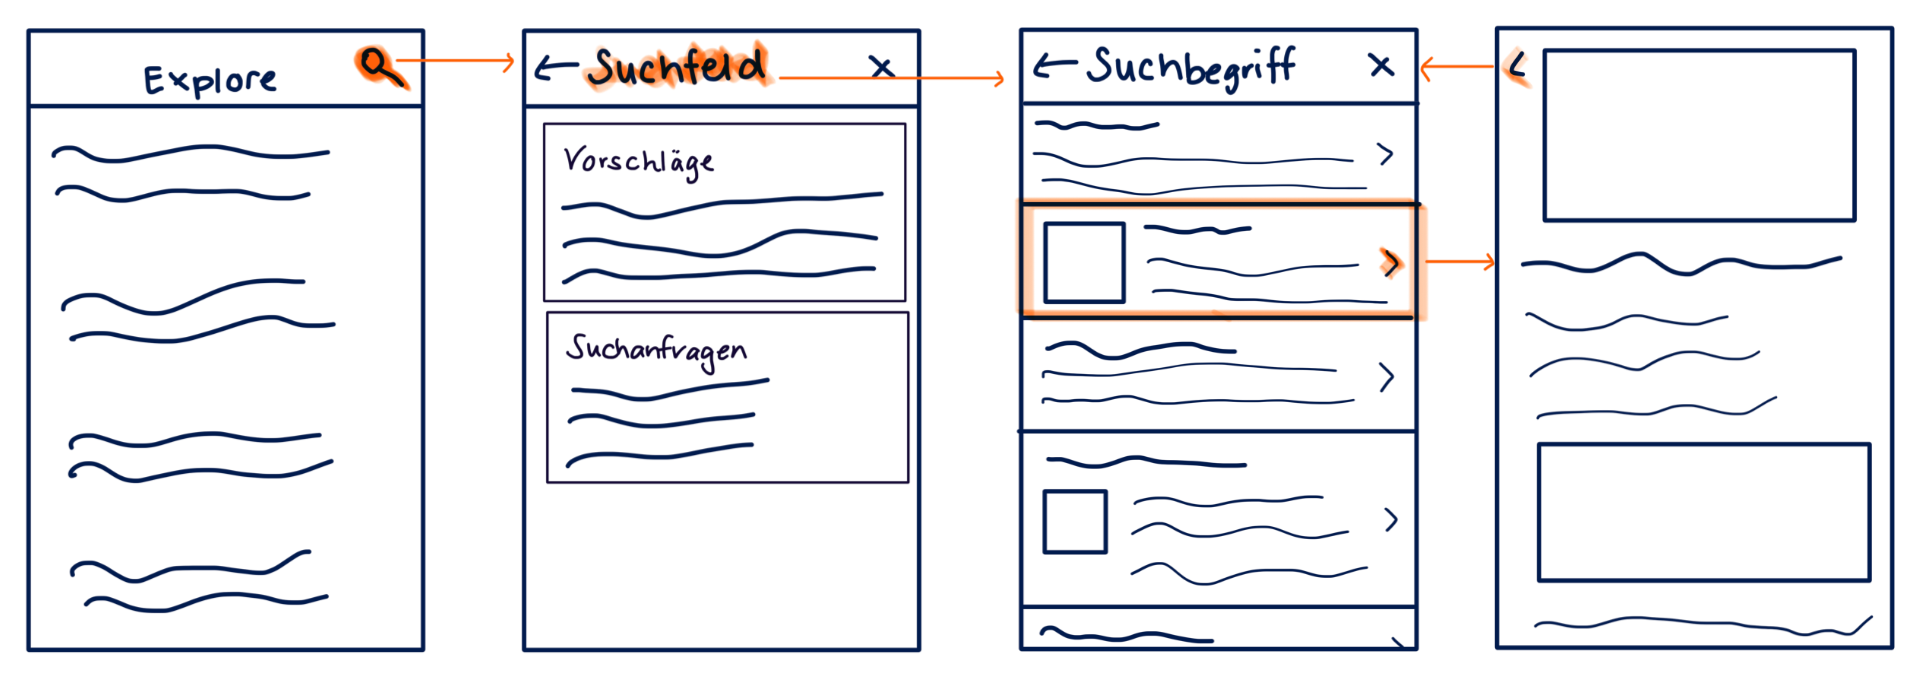
\includegraphics[width=1\linewidth,height=\textheight,keepaspectratio]{source/figures/Wireframes_ba_1.png}
\caption{Quelle: eigene Zeichnung, 2025}\label{fig:wireframe_1}
\end{figure}

Der Suchbegriff wird durch Ausführen der Suche an die API übergeben, die
nach der Verarbeitung die passenden Ergebnisse aus den verschiedenen
Quellen zurückgibt. Diese werden dann untereinander aufgelistet, wobei
die verschiedenen Ergebnisse deutlich voneinander unterschieden werden.
Die eigentliche Suchfunktion liegt also in der API, die im folgenden
Kapitel konzipiert wird.

\section{Konzeption der API}\label{konzeption-der-api}

Nachdem im vorherigen Kapitel das Bedienkonzept erarbeitet worden ist,
soll nun die bisher nicht näher betrachtete API konzipiert werden. Die
hier zu entwickelnde API wird als Schnittstelle in das existierende
App-Umfeld hinzugefügt.

\subsection{Schnittstellen-Design}\label{schnittstellen-design}

Der Zugriff auf die API erfolgt über einen lokalen Aufruf innerhalb der
Suchfunktion. Bei Bestätigung der Eingabe in das Suchfeld wird der
Suchbegriff an die Schnittstelle übergeben. Als Rückgabewert werden dann
die Ergebnisse der Suche erwartet.

Um die Daten auslesen zu können, muss die API auf verschiedene
Datenquellen zugreifen. Für die prototypische Umsetzung sind die
\emph{`String-Files'-}, \emph{Kontext-} und \emph{Lokale-Daten}. Die
detaillierte Betrachtung des Zugriffs auf diese Daten erfolgt in Kapitel
\ref{implementierung-der-api}.

\subsection{Architektur-Entwurf}\label{architektur-entwurf}

Infos in {[}@nunkesserAppEntwicklungFuerMobile2023{]} ab Seite 65

Aufbau:

\begin{itemize}
\tightlist
\item
  Architekturübersicht

  \begin{itemize}
  \tightlist
  \item
    Auteilung in Searchable und Findable
  \item
    in API für jede Quelle: Provider
  \item
    wichtig: theoretisch ausbaubar! -\textgreater{} Skalierbarkeit
  \end{itemize}
\item
  Datenfluss erklären

  \begin{itemize}
  \tightlist
  \item
    für jede Quelle den Datenfluss erklären
  \end{itemize}
\end{itemize}

\chapter{Implementierung der API und
Suchfunktion}\label{implementierung-der-api-und-suchfunktion}

\section{Implementierung der API}\label{implementierung-der-api}

\subsection{Vertiefte Hintergründe der
API}\label{vertiefte-hintergruxfcnde-der-api}

\section{Implementierung des
Suchfunktions-Prototyps}\label{implementierung-des-suchfunktions-prototyps}

\section{Benutzeroberfläche}\label{benutzeroberfluxe4che}

Mehr in Quelle {[}@nunkesserAppEntwicklungFuerMobile2023{]} ab Seite 122
\ldots{}

Quelle {[}@richterUsabilityUndUX2016{]}: User Experience Definition:
``User Experience (UX): Hier steht das Gesamterlebnis der Benutzer bei
der Verwendung von Produkten, Systemen und Diensten im Fokus. Nebst den
funktionalen Aspekten werden dabei vermehrt auch emotionale und
ästhetische Faktoren berücksichtigt. So liegt neben geschäftlichen
Anwendungen ein Schwerpunkt des Gebietes auf Lösungen und Produkten im
Consumer-Bereich, also etwa auf E-Services, Smartphone Apps und
digitalen Geräten, aber auch für Spiele und Anwendungen im
Unterhaltungsbereich spielen die genannten Faktoren eine entscheidende
Rolle für den Produkterfolg. Aufgrund der umfassenderen
Betrachtungsweise hat der Begriff UX sich in vielfältiger Weise
durchgesetzt und löst immer mehr auch die Bezeichnung Usability als
Qualitätsbegriff ab.'' + Mehr auf Seite 12 + Seite 14 Tabelle

Quelle {[}@deeBestPracticesInapp2024{]}:

\chapter{Evaluierung}\label{evaluierung}

\section{Anforderungsabgleich}\label{anforderungsabgleich}

\section{Bewertung des Konzepts anhand von
Beispielszenarien}\label{bewertung-des-konzepts-anhand-von-beispielszenarien}

\section{Evaluierung der
Suchfunktion}\label{evaluierung-der-suchfunktion}

\subsection{Evaluierung der
Suchergebnisse}\label{evaluierung-der-suchergebnisse}

\subsection{Nutzerbefragung zur
Suchfunktion}\label{nutzerbefragung-zur-suchfunktion}

Infos zur Nutzerbefragung: {[}@richterUsabilityUndUX2016{]}: -
Benutzerbefragungen mit Fragebögen sind wichtige Methode, um Antworten
von einer größeren Anzahl Personen zu erhalten (sic) - Fragebögen werden
zur Analyse von Benutzern und Kontext, und zur Beurteilung eines Systems
(Evaluation) eingesetzt - quantitative Studie, weil Antworten mit
Fragebogen zählbar sind - Für Erkenntisse in Usability und UX oke, aber
eig immer hinterfragen, ob Usability-Tests oder Experten-Reviews nicht
besser wäre - wichtig: Vergleichbarkeit: Ergebnisse können verdichtet,
statistisch ausgewertet und miteinander verglichen werden - Gut für
Beurteilung von verschiedenen Systemen -

Mehr Infos: {[}@butzMenschMaschineInteraktion2022{]} Seite 125 - 130

\section{Vergleich mit Daten}\label{vergleich-mit-daten}

Aufnahme mit ``{[}@Referenz{]}''

kursiv: * auf beiden Seiten des Textes -\textgreater{} \emph{kursiv}
fett: ** -\textgreater{} \textbf{fett} kursiv und fett: ***
--\textgreater{} \textbf{\emph{fett und kursiv}}

Aenean nec dapibus in mL/min\textsuperscript{-1}. Mathematical formula
can be inserted using Latex:

\begin{enumerate}
\def\labelenumi{(\arabic{enumi})}
\tightlist
\item
  \(f(x) = ax^3 + bx^2 + cx + d\)
\end{enumerate}

Die Tabelle \ref{tabellenreferenz} zeigt uns wie man eine Tabelle
hinzufügt.

\begin{itemize}
\tightlist
\item
  erstes Element der Liste
\item
  zweites Element der Liste
\item
  drittes Element der Liste
\end{itemize}

\begin{enumerate}
\def\labelenumi{\arabic{enumi}.}
\tightlist
\item
  erstes Element
\item
  zweites Element
\item
  drittes Element
\end{enumerate}

Syntaxhervorhebung in Codeblöcken erreicht man mit drei ``\,`'' Zeichen
vor und nach dem Codeblock.

\begin{Shaded}
\begin{Highlighting}[]
\NormalTok{mood }\OperatorTok{=} \StringTok{\textquotesingle{}happy\textquotesingle{}}
\ControlFlowTok{if}\NormalTok{ mood }\OperatorTok{==} \StringTok{\textquotesingle{}happy\textquotesingle{}}\NormalTok{:}
    \BuiltInTok{print}\NormalTok{(}\StringTok{"I am a happy robot"}\NormalTok{)}
\end{Highlighting}
\end{Shaded}

Die Tabelle \ref{tabellenreferenz} zeigt uns wie man eine Tabelle
hinzufügt. Integer tincidunt sed nisl eget pellentesque. Mauris
eleifend, nisl non lobortis fringilla, sapien eros aliquet orci, vitae
pretium massa neque eu turpis. Pellentesque tincidunt aliquet volutpat.
Ut ornare dui id ex sodales laoreet.

\newpage

\begin{longtable}[]{@{}
  >{\raggedright\arraybackslash}p{(\linewidth - 4\tabcolsep) * \real{0.2778}}
  >{\raggedright\arraybackslash}p{(\linewidth - 4\tabcolsep) * \real{0.3333}}
  >{\raggedright\arraybackslash}p{(\linewidth - 4\tabcolsep) * \real{0.2778}}@{}}
\caption{Das ist die Tabellenbeschriftung. Suspendisse blandit dolor sed
tellus venenatis, venenatis fringilla turpis pretium.
\label{tabellenreferenz}}\tabularnewline
\toprule\noalign{}
\begin{minipage}[b]{\linewidth}\raggedright
Spalte 1
\end{minipage} & \begin{minipage}[b]{\linewidth}\raggedright
Spalte 2
\end{minipage} & \begin{minipage}[b]{\linewidth}\raggedright
Spalte 3
\end{minipage} \\
\midrule\noalign{}
\endfirsthead
\toprule\noalign{}
\begin{minipage}[b]{\linewidth}\raggedright
Spalte 1
\end{minipage} & \begin{minipage}[b]{\linewidth}\raggedright
Spalte 2
\end{minipage} & \begin{minipage}[b]{\linewidth}\raggedright
Spalte 3
\end{minipage} \\
\midrule\noalign{}
\endhead
\bottomrule\noalign{}
\endlastfoot
Zeile 1 & 0.1 & 0.2 \\
Zeile 2 & 0.3 & 0.3 \\
Zeile 3 & 0.4 & 0.4 \\
Zeile 4 & 0.5 & 0.6 \\
\end{longtable}

\chapter{Fazit}\label{fazit}

\section{Zusammenfassung der Arbeit}\label{zusammenfassung-der-arbeit}

Zusammenfassend

\section{Ausblick}\label{ausblick}

Es gibt mehrere mögliche Richtungen, um diese Arbeit zu erweitern.

Mehr Funktionen: - Suchwort im Text markieren - Filter: Quellen
ausschließen / wählen - Suche mit kontextuellen Daten: -
{[}@yndurainAugmentingMobileSearch2012{]} -\textgreater{} Such data can
provide more meaningful search results by augmenting searches with
real-world information related to users' profiles and behavioral
patterns. Information about users such as location, how they interact
with the mobile device, or what's occurring in the surrounding physical
world is called contextual data. Such information is increasingly
accessible via sensors embedded in smartphones leading to many new
commercial usage scenarios --- such as location-based services --- and
academic research on the topic. \ldots{} - Context Awareness: The term
context, or context awareness, usually refers to a general class of
systems that can sense a continuously changing physical environment and
provide relevant services to users on this basis - Im mobilen Context: •
signal coverage strength; • active connectivity methods; • environmental
information, such as light; • current location; • activity time and time
frame; • internal device information, such as power; and • the device's
motion and angle.

\chapter*{Anhang 1: Einige Extras}\label{anhang-1-einige-extras}
\addcontentsline{toc}{chapter}{Anhang 1: Einige Extras}

Füge Anhang 1 hier hinzu.

\chapter*{Anhang 2: Noch mehr Extras}\label{anhang-2-noch-mehr-extras}
\addcontentsline{toc}{chapter}{Anhang 2: Noch mehr Extras}

Füge Anhang 2 hier hinzu.

\footnotesize

\chapter{Literatur}\label{literatur}

\end{document}
